% TODO:














%%%%%%%%%%%%%%%%%%%%%%%%%%%%%%%%%%%%%%%%%
% Beamer Presentation
% LaTeX Template
% Version 1.0 (10/11/12)
%
% This template has been downloaded from:
% http://www.LaTeXTemplates.com
%
% License:
% CC BY-NC-SA 3.0 (http://creativecommons.org/licenses/by-nc-sa/3.0/)
%
%%%%%%%%%%%%%%%%%%%%%%%%%%%%%%%%%%%%%%%%%

%----------------------------------------------------------------------------------------
%	PACKAGES AND THEMES
%----------------------------------------------------------------------------------------

\documentclass{beamer}

\mode<presentation> {

% The Beamer class comes with a number of default slide themes
% which change the colors and layouts of slides. Below this is a list
% of all the themes, uncomment each in turn to see what they look like.

%\usetheme{default}
%\usetheme{AnnArbor}
%\usetheme{Antibes}
%\usetheme{Bergen}
%\usetheme{Berkeley}
%\usetheme{Berlin}
%\usetheme{Boadilla}
%\usetheme{CambridgeUS}
%\usetheme{Copenhagen}
%\usetheme{Darmstadt}
%\usetheme{Dresden}
%\usetheme{Frankfurt}
%\usetheme{Goettingen}
%\usetheme{Hannover}
%\usetheme{Ilmenau}
%\usetheme{JuanLesPins}
%\usetheme{Luebeck}
\usetheme{Madrid}
%\usetheme{Malmoe}
%\usetheme{Marburg}
%\usetheme{Montpellier}
%\usetheme{PaloAlto}
%\usetheme{Pittsburgh}
%\usetheme{Rochester}
%\usetheme{Singapore}
%\usetheme{Szeged}
%\usetheme{Warsaw}

% As well as themes, the Beamer class has a number of color themes
% for any slide theme. Uncomment each of these in turn to see how it
% changes the colors of your current slide theme.

%\usecolortheme{albatross}
%\usecolortheme{beaver}
%\usecolortheme{beetle}
%\usecolortheme{crane}
%\usecolortheme{dolphin}
%\usecolortheme{dove}
%\usecolortheme{fly}
%\usecolortheme{lily}
%\usecolortheme{orchid}
%\usecolortheme{rose}
%\usecolortheme{seagull}
%\usecolortheme{seahorse}
%\usecolortheme{whale}
%\usecolortheme{wolverine}

%\setbeamertemplate{footline} % To remove the footer line in all slides uncomment this line
%\setbeamertemplate{footline}[page number] % To replace the footer line in all slides with a simple slide count uncomment this line

%\setbeamertemplate{navigation symbols}{} % To remove the navigation symbols from the bottom of all slides uncomment this line
}

\usepackage[utf8]{inputenc}
\usepackage[russian]{babel}
\usepackage{cmap}


\usepackage{verbatim}
\usepackage{fancybox}
\usepackage{ulem}
\usepackage{tikz}
\usetikzlibrary{positioning}
\usepackage{scalefnt}
\usetikzlibrary{arrows,shapes,positioning,shadows,trees,calc,backgrounds,fit,positioning}

\usepackage{graphicx} % Allows including images
\usepackage{booktabs} % Allows the use of \toprule, \midrule and \bottomrule in tables
\usepackage{textcomp}
\usepackage{listings}
\usepackage{color}
\usepackage{xcolor}
\usepackage{changepage}
\usepackage{multicol}

\definecolor{mygreen}{rgb}{0,0.6,0}
\definecolor{mygray}{rgb}{0.5,0.5,0.5}
\definecolor{mymauve}{rgb}{0.58,0,0.82}

\lstset{ %
  backgroundcolor=\color{white},   % choose the background color; you must add \usepackage{color} or \usepackage{xcolor}
  basicstyle=\footnotesize,        % the size of the fonts that are used for the code
  breakatwhitespace=false,         % sets if automatic breaks should only happen at whitespace
  breaklines=true,                 % sets automatic line breaking
  captionpos=b,                    % sets the caption-position to bottom
  commentstyle=\color{mygreen},    % comment style
  deletekeywords={...},            % if you want to delete keywords from the given language
  escapeinside={\%*}{*)},          % if you want to add LaTeX within your code
  extendedchars=true,              % lets you use non-ASCII characters; for 8-bits encodings only, does not work with UTF-8
  frame=single,                    % adds a frame around the code
  keepspaces=true,                 % keeps spaces in text, useful for keeping indentation of code (possibly needs columns=flexible)
  keywordstyle=\color{blue},       % keyword style
  language=Octave,                 % the language of the code
  morekeywords={*,...},            % if you want to add more keywords to the set
  numbers=left,                    % where to put the line-numbers; possible values are (none, left, right)
  numbersep=5pt,                   % how far the line-numbers are from the code
  numberstyle=\tiny\color{mygray}, % the style that is used for the line-numbers
  rulecolor=\color{black},         % if not set, the frame-color may be changed on line-breaks within not-black text (e.g. comments (green here))
  showspaces=false,                % show spaces everywhere adding particular underscores; it overrides 'showstringspaces'
  showstringspaces=false,          % underline spaces within strings only
  showtabs=true,                  % show tabs within strings adding particular underscores
  stepnumber=1,                    % the step between two line-numbers. If it's 1, each line will be numbered
  stringstyle=\color{mymauve},     % string literal style
  tabsize=4,                       % sets default tabsize to 2 spaces
  %title=\lstname                   % show the filename of files included with \lstinputlisting; also try caption instead of title
}

\graphicspath{{./figures/}}

%----------------------------------------------------------------------------------------
%	TITLE PAGE
%----------------------------------------------------------------------------------------

\title[Обработка и исполнение запросов: лекция 5]{Обработка и исполнение запросов в СУБД (Лекция 5) \\~\\ Классические системы: принципы построения распределенных СУБД\\~\\ v5} % The short title appears at the bottom of every slide, the full title is only on the title page

\author{Георгий Чернышев} % Your name
\institute[ВШЭ] % Your institution as it will appear on the bottom of every slide, may be shorthand to save space
{
Высшая Школа Экономики \\ % Your institution for the title page
\medskip
\textit{chernishev@gmail.com} % Your email address
}
%\date{\today} % Date, can be changed to a custom date

\date{30 сентября 2020 г.}

\begin{document}

\begin{frame}
\titlepage % Print the title page as the first slide
\end{frame}

\begin{comment}
\begin{frame}
\frametitle{Overview} % Table of contents slide, comment this block out to remove it
\tableofcontents % Throughout your presentation, if you choose to use \section{} and \subsection{} commands, these will automatically be printed on this slide as an overview of your presentation
\end{frame}
\end{comment}

\begin{frame}
\frametitle{РСУБД: что нового по сравнению с централизованной?}

\begin{figure}[htb]
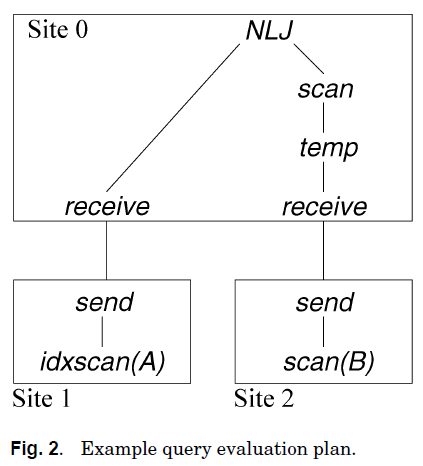
\includegraphics[width=\textwidth,height=0.80\textheight,keepaspectratio]{kossman-2.png} 
\footnote{\tiny{Изображение взято из \cite{Kossmann2000}}}
\end{figure}

\end{frame}

\begin{frame}
\frametitle{Распределенная оптимизация}

\begin{itemize}
  \setlength\itemsep{1em}
  \item Отношения могут быть реплицированы и копии могут быть размещены на разных узлах;
  
  \item Выбирать AM можно с помощью алгоритма динамического программирования (см. лекцию 2), но теперь не просто $scan(A)$, а $scan(A, S_1)$ и $scan(A, S_2)$. Теперь нельзя сразу же отбрасывать по стоимости~--- результаты получаются на разных узлах!

  \item Соединения также производят результаты на разных узлах $\longrightarrow$ концепция interesting sites, аналог interesting orders. 
  
  \item Выигрыш от кустистых планов выше в распределенных системах.
\end{itemize}
$\longrightarrow$ оптимизация сложнее нежели в централизованных системах

\end{frame}


\begin{frame}
\frametitle{Стоимостные модели для распределенной оптимизации}

\begin{itemize}
  \setlength\itemsep{1em}
  \item Модель потребления ресурсов:
  \begin{itemize}
    \item Централизованная система: \\
    CPU + disk I/O;
    \item Распределенная: \\
    CPU + disk I/O + network I/O + packing/unpacking + ...;
    \item Линейная комбинация с весами;
  \end{itemize}

  \item Модель времени ответа:
  \begin{itemize}
    \item Иногда нужен быстрый ответ $\longrightarrow$ нужен внутризапросный параллелизм;
    \item Модель учитывает: 
    \begin{itemize}
    	\item независимый внутризапросный параллелизм, и,
    	\item pipelining параллелизм (aka неблокирующие операторы, лекция 1).
    \end{itemize}
    
  \end{itemize}
  
\end{itemize}

Конкретные примеры моделей есть в 8 главе \cite{Ozsu2011}.

\end{frame}

\begin{frame}
\frametitle{Две модели: пример}

\begin{figure}[htb]
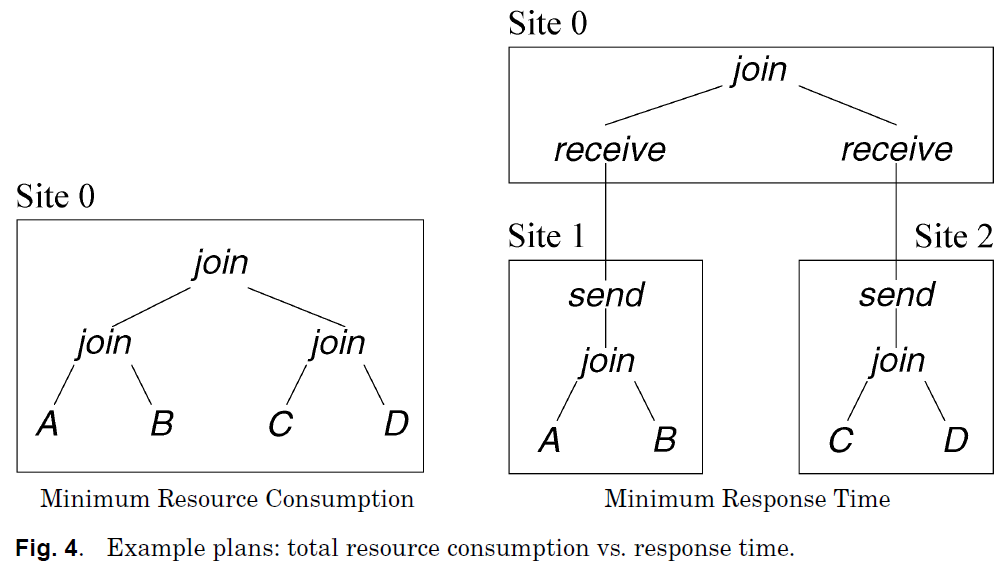
\includegraphics[width=\textwidth,height=0.80\textheight,keepaspectratio]{kossman-3.png} 
\footnote{\tiny{Изображение взято из \cite{Kossmann2000}}}
\end{figure}

\end{frame}

\begin{frame}
	\frametitle{Две модели: независимый внутризапросный параллелизм}
	
	\begin{figure}[htb]
		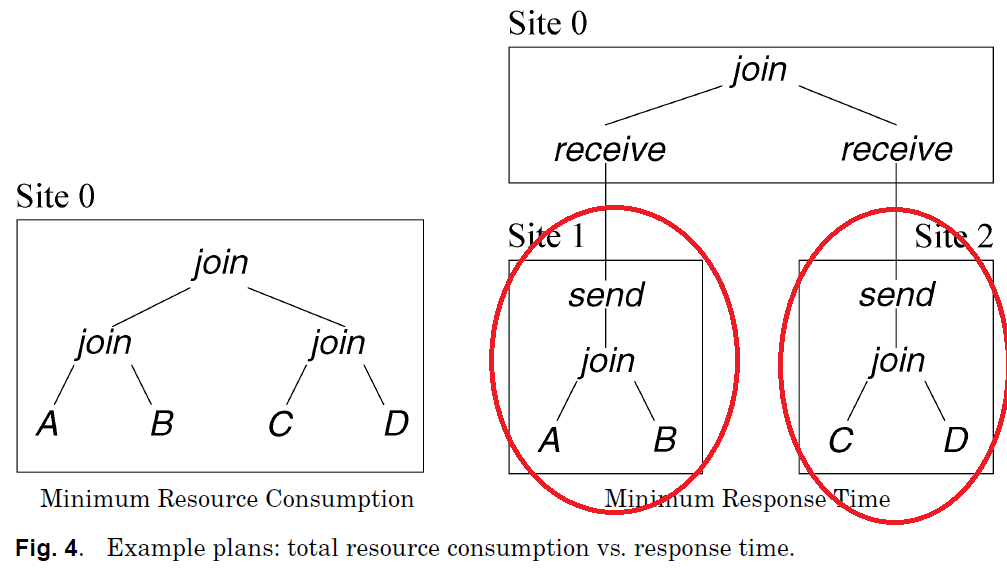
\includegraphics[width=\textwidth,height=0.80\textheight,keepaspectratio]{kossman-3a.png} 
		\footnote{\tiny{Изображение взято из \cite{Kossmann2000}}}
	\end{figure}
	
\end{frame}

\begin{frame}
	\frametitle{Две модели: pipelining параллелизм}
	
	\begin{figure}[htb]
		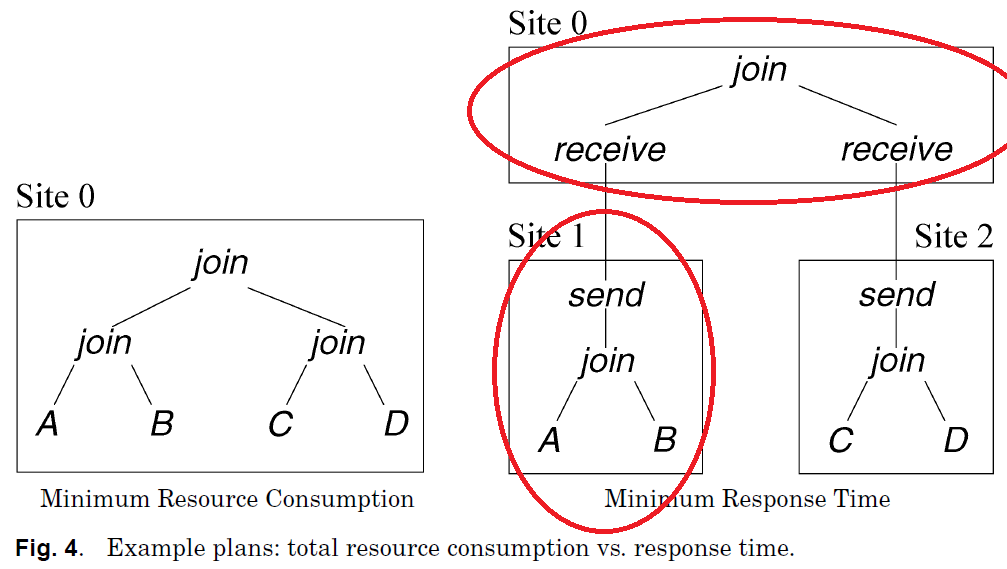
\includegraphics[width=\textwidth,height=0.80\textheight,keepaspectratio]{kossman-3b.png} 
		\footnote{\tiny{Изображение взято из \cite{Kossmann2000}}}
	\end{figure}
	
\end{frame}

\begin{frame}
\frametitle{``Наивная'' модель времени ответа}

\begin{enumerate}
  \setlength\itemsep{1em}
  \item Вычисляем сколько потребит каждый оператор в отдельности;
  \item Вычисляется использование разделяемого ресурса всеми операторами работающими параллельно. Это делается для каждого ресурса.
  \begin{itemize}
    \item Пример: сеть. Пропускная способность сети делится на суммарный объем переданных данных (который передали все операторы).
  \end{itemize}
  \item  Время ответа группы операторов вычисляется как \alert{максимум} по потреблению ресурсов отдельных операторов (каждого) и всех разделяемых ресурсов.
\end{enumerate}

\end{frame}


\begin{frame}
\frametitle{Пример}

Предположим:
\begin{enumerate}
  \setlength\itemsep{1em}
  \item На каждом узле по одному процессору, с одним ядром;
  \item Все соединения во всех планах работают параллельно (поточно или нет);
  \item Каждый оператор соединения стоит 200 секунд работы CPU и нет disk I/O;
  \item У сети нет задержек, доставка $A \bowtie B$ и $C \bowtie D$ стоят 130 секунд работы сети (каждая);
  \item Посылка и получение данных в/из сети ничего не стоит;
  \item Чтение всех таблиц с диска ничего не стоит;
\end{enumerate}

\end{frame}

\begin{frame}
\frametitle{Пример, продолжение}

Тогда:
\begin{enumerate}
  \setlength\itemsep{1em}
  \item Время работы левого плана будет $600$ секунд (CPU только);
  \item Время работы правого плана будет $max (130 + 130, 200, 200, 200) = 260$;
\end{enumerate}

Всё хорошо, однако: 
\begin{itemize}
  \setlength\itemsep{1em}
  \item не учитывается scheduling и конкуренция за ресурс: что будет если на узел оптимизатор бросит сразу много операторов из разных запросов?
\end{itemize}

Преимущество: модель дешева в использовании.

\end{frame}


\begin{frame}[allowframebreaks]
\frametitle{Как исполнять запросы?}

Набор приемов для построения (минимально) эффективной РСУБД: 
\begin{itemize}
  \setlength\itemsep{1em}
  \item Поблочная передача данных (нужно настраивать под размер сообщения, учет алгоритма Нагеля и прочее);
  \item Оптимизация мультикастов: выбор оптимального маршрута передачи;
  \item Уместное использование многопоточности:

  \begin{figure}[htb]
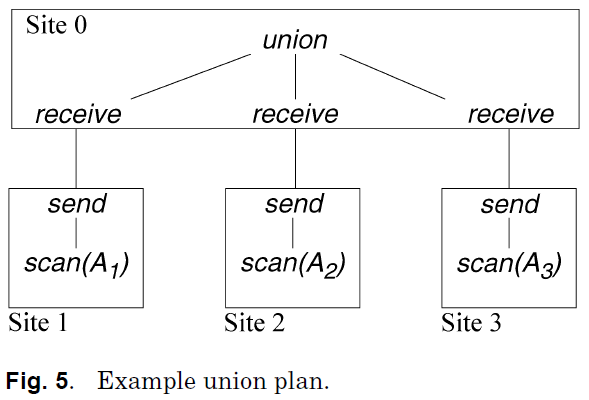
\includegraphics[width=\textwidth,height=0.35\textheight,keepaspectratio]{kossman-4.png} 
\footnote{\tiny{Изображение взято из \cite{Kossmann2000}}}
\end{figure}  
\end{itemize}


\begin{itemize}
  \setlength\itemsep{1em}

  \item \alert{Неуместное} использование многопоточности:

  \begin{figure}[htb]
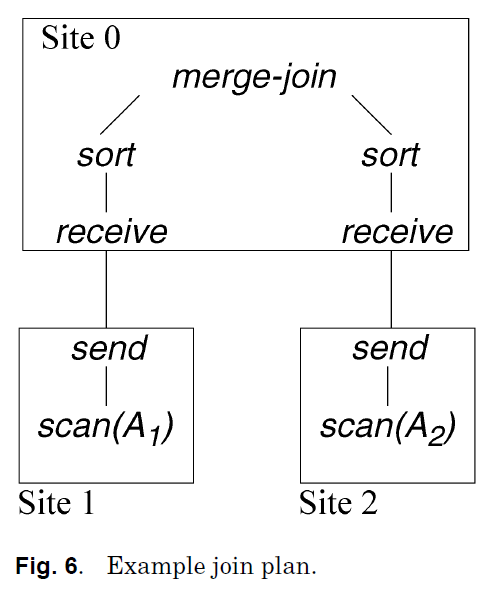
\includegraphics[width=\textwidth,height=0.35\textheight,keepaspectratio]{kossman-5.png} 
\footnote{\tiny{Изображение взято из \cite{Kossmann2000}}}

Если не повезет, потоки будут драться за НМЖД (disk thrashing).

\end{figure}  


  \item Горизонтальное фрагментирование + репликация: \\
  Пусть $ A = A_1 \cup A_2$, надо $A \bowtie B$
  \begin{itemize}
    \item Тогда: $(A_1 \cup A_2) \bowtie B$ или $(A_1 \bowtie B) \cup (A_2 \bowtie B)$
    \item Иногда можно и так: $((A_1 \cup A_2) \bowtie B) \cup (A_3 \bowtie B)$
  \end{itemize}
  
\end{itemize}

\end{frame}

\begin{frame}
\frametitle{Как исполнять запросы? III}

\begin{itemize}
  \setlength\itemsep{1em}

  \item Попарно не пересекающиеся фрагменты отношений: 
  $$(Emp_1 \cup Emp_2 ... \cup EMP_n) \bowtie (Dept_1 \cup Dept_2 ... \cup Dept_n) =$$ $$(Emp_1 \bowtie Dept_1) \cup (Emp_2 \bowtie Dept_2) ... \cup (Emp_n \bowtie Dept_n)$$
  
  Чтобы это работало нужно правильно фрагментировать, иначе~--- каждый с каждым.
  
  \item Другие реализации параллельного соединения \cite{Taniar2008}.

  \item Трюк с полусоединением: таблицы $A$ и $B$ на разных узлах \\
  $$A \bowtie B = A \bowtie (B \ltimes \pi (A))$$

  На самом деле всё не так просто, возможных планов с полусоединением~--- много, см. 8 главу \cite{Ozsu2011}.

  \item Double-pipelined hash join: борьба с неравномерностью нагрузки.

\end{itemize}

\end{frame}


\begin{frame}
\frametitle{Как исполнять запросы? IV}

\begin{itemize}
  \setlength\itemsep{1em}

  \item Оператор stop для SELECT TOP

    \begin{figure}[htb]
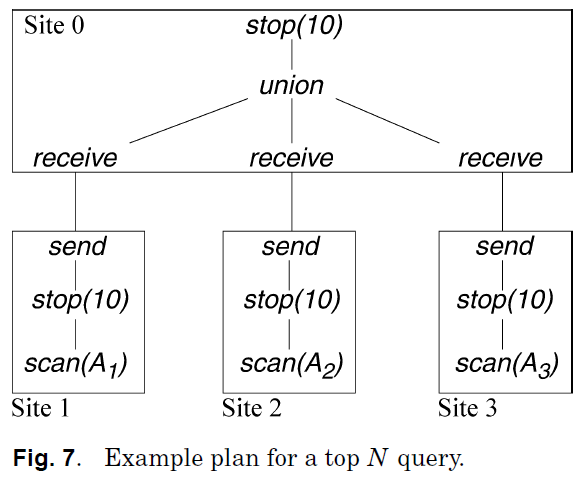
\includegraphics[width=\textwidth,height=0.75\textheight,keepaspectratio]{kossman-6.png} 
\footnote{\tiny{Изображение взято из \cite{Kossmann2000}}}
 \end{figure}    

\end{itemize}

\end{frame}

\begin{frame}
\frametitle{Как исполнять запросы? V}

\begin{itemize}
  \setlength\itemsep{1em}

  \item Мультимедиа РСУБД, пусть надо выполнить TOP(N) и известно что функция оценки~--- монотонная функция\\~\\например, найти TOP 10 от\\~\\ f (voice, score) = score(voice) + score(looks) ORDERBY ASCENDING\\~\\
  тогда работает такой алгоритм:
  \begin{itemize}
    \item Последовательно просим top от voice и looks, пока пересечение не будет иметь 10 объектов;
    \item Вычисляем ранжирующую функцию $f$ для тех птиц, что не входят в пересечение и выдаем результат.
  \end{itemize}
  
\end{itemize}

Монотонность: если $s_1(a)<s_1(b)$ и $s_2(a)<s_2(b)$ означает $f(s_1(a),
s_2(a)) < f(s_1(b), s_2(b))$.

\end{frame}

\begin{frame}
\frametitle{Как исполнять запросы? VI}

Пример (TOP 2):

\begin{multicols}{2}
\begin{center}
	\begin{tabular}{ | c | c | }
		\hline
		looks & score  \\ \hline
		\alert{\textbf{a 1}} & \alert{e 2} \\ \hline
		\alert{\textbf{b 2}} & \alert{f 3} \\ \hline
		\alert{c 3} & \alert{\textbf{a 8}} \\ \hline
		\alert{d 3} & \alert{\textbf{b 9}} \\ \hline
		e 3.5       & c 10 \\ \hline        
		f 3.8       & d 11 \\ \hline
		... & ... \\ \hline
	\end{tabular}
\end{center}
	\columnbreak
a = 1 + 8 = 9\\
b = 2 + 9 = 11\\
c = 3 + 10 = 13\\
d = 3 + 11 = 14\\
\alert{e = 3.5 + 2 = 5.5}\\
\alert{f = 3.8 + 3 = 6.8}
	
\end{multicols}


\end{frame}

\begin{frame}
\frametitle{Клиент-серверные системы}

Система где разделяются типы машин (см. предыдущую лекцию): обслуживающие запросы и хранящие данные.\\~\\

Основные вопросы:

\begin{itemize}
  \setlength\itemsep{1em}

  \item Выполнять запрос на машине где находятся данные или же на клиенте?
  \item Как использовать кеширование на клиентах?

\end{itemize}

\end{frame}


\begin{frame}
\frametitle{Выполнение запросов в клиент-серверных системах}

\begin{multicols}{2}

\begin{figure}[htb]
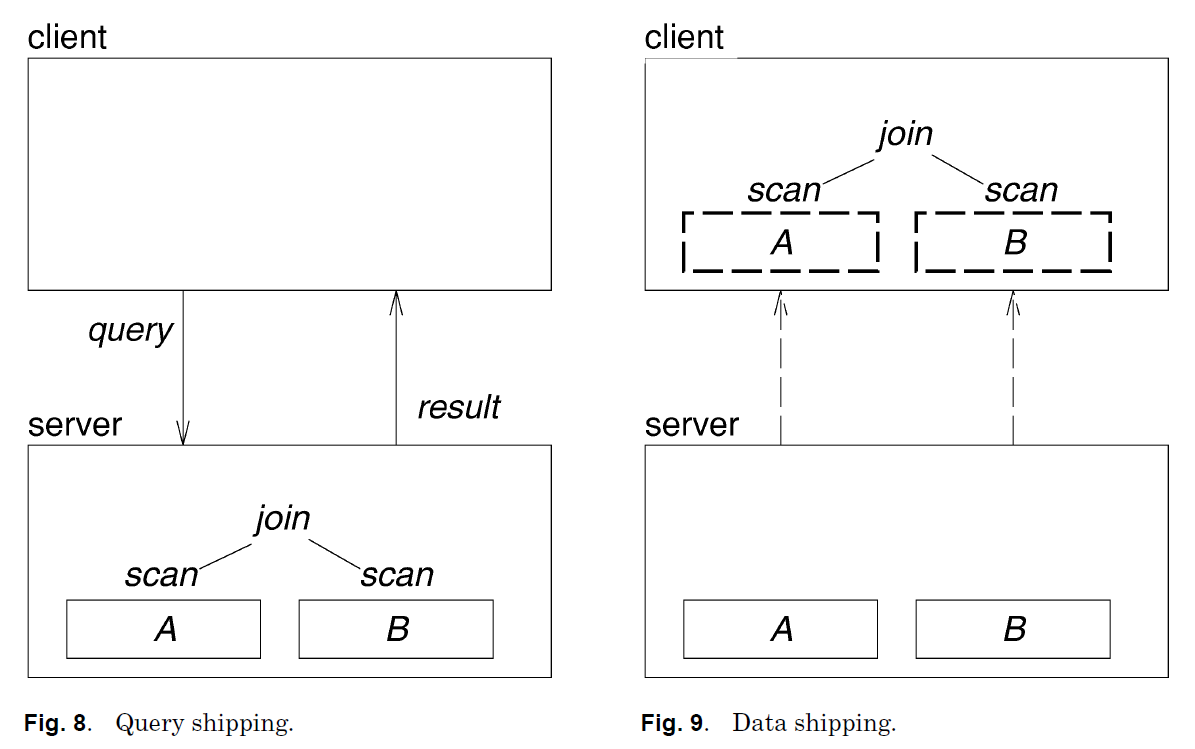
\includegraphics[width=\textwidth,height=0.35\textheight,keepaspectratio]{kossman-7.png} 
 \end{figure} 
	\columnbreak
   
\begin{figure}[htb]
	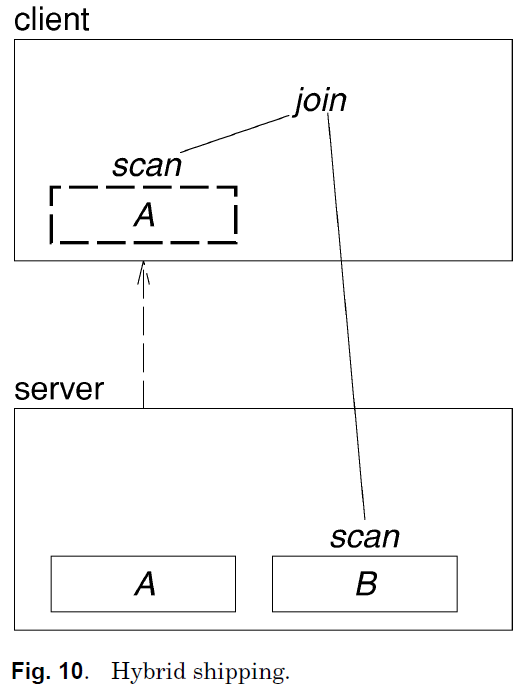
\includegraphics[width=\textwidth,height=0.35\textheight,keepaspectratio]{kossman-7a.png} 
	\footnote{\tiny{Изображение взято из \cite{Kossmann2000}}}
\end{figure}    
\end{multicols}

Стратегии:
\begin{itemize}
  \setlength\itemsep{1em}

  \item Миграция данных (data shipping);
  \item Миграция запроса (query shipping);
  \item Гибридная (hybrid shipping).
\end{itemize}
\end{frame}


\begin{frame}
\frametitle{Что лучше?}

\begin{itemize}
  \setlength\itemsep{1em}

  \item Зависит от машин: каждая из схем имеет свою нишу;
  \item В гибридных оптимизация сложнее;
  \item Иногда выгодно игнорировать кеши на клиентах: две выборки, соединение и быстрая сеть;
  \item Иногда выгодно ``вернуть'' (промежуточные) данные на сервер: быстрая сеть, сервер эффективно обрабатывает соединения;
  \item Маленькие апдейты хранить на клиентах, а большие на серверах.
\end{itemize}
\end{frame}

\begin{comment}
\begin{frame}
\frametitle{Оптимизация в РСУБД I}

Выбор места выполнения оператора:

\begin{figure}[htb]
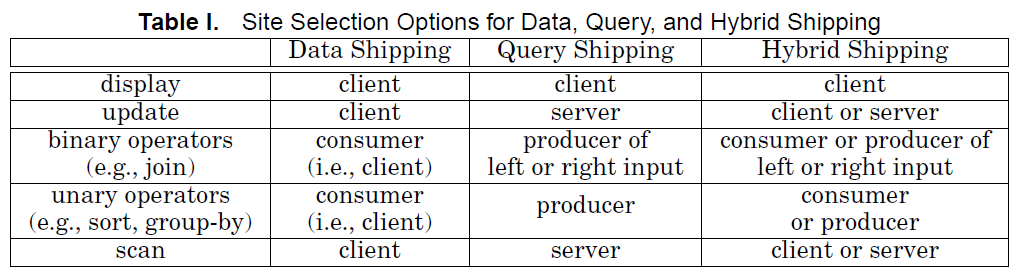
\includegraphics[width=\textwidth,height=0.75\textheight,keepaspectratio]{kossman-8.png} 
\footnote{\tiny{Изображение взято из \cite{Kossmann2000}}}
 \end{figure}    

Аннотации транслируются в адреса машин, затем им ``раздается'' код.\\~\\

Если есть репликация то можно повыбирать.

\end{frame}
\end{comment}


\begin{frame}
\frametitle{Оптимизация в РСУБД}

Когда и где оптимизировать? Мнений много, некоторые мысли:

\begin{itemize}
  \setlength\itemsep{1em}

  \item Разбор и перезапись запроса лучше делать на клиенте: разгружаем сервер. Оптимизация~--- на сервере: понятно если он один, иначе выбор через эвристику.
  \item Оптимизация на сервере в случае когда их несколько: спрашивать состояние vs угадывать состояние.
  \item Подходы к оптимизации запросов: сохраненные планы запросов, набор альтернативных планов, реоптимизация, ...
  \item Двухшаговая оптимизация~--- самый популярный подход:
  \begin{enumerate}
    \setlength\itemsep{1em}
    \item абстрактный план: access methods, порядок соединений;
    \item прямо перед выполнением трансформировать план и выбирать узлы.
  \end{enumerate}
\end{itemize}


\end{frame}


\begin{frame}
\frametitle{Свойства двухшагового подхода}

Плюсы:
\begin{itemize}
  %\setlength\itemsep{1em}

  \item Каждый шаг дешев;
  \item Второй шаг позволяет делать load-balancing;
  \item Второй шаг позволяет использовать кеширование.
\end{itemize}

Минусы:
\begin{itemize}
  \setlength\itemsep{1em}
  \item Неоптимальные планы с точки зрения сетевой стоимости.
\end{itemize}

\begin{figure}[htb]
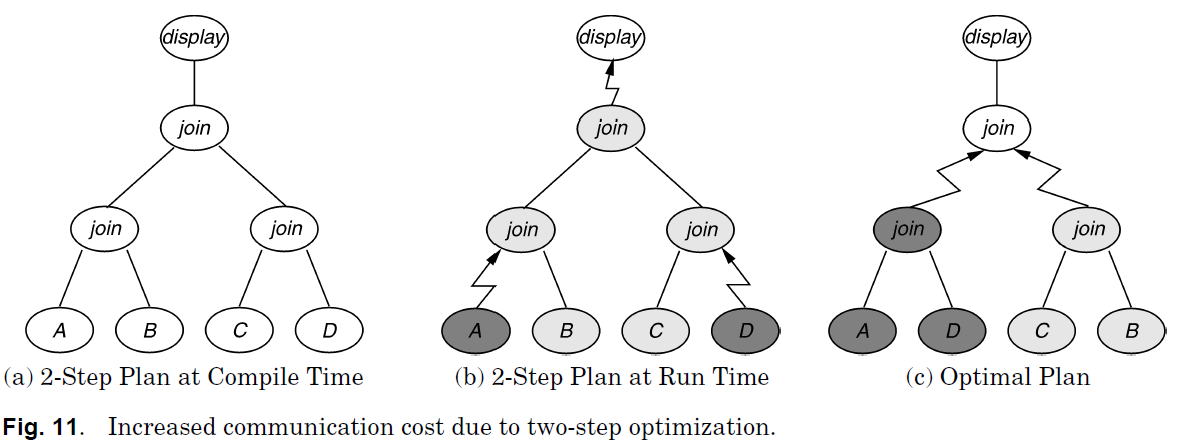
\includegraphics[width=\textwidth,height=0.65\textheight,keepaspectratio]{kossman-9.png} 
\footnote{\tiny{Изображение взято из \cite{Kossmann2000}}}
 \end{figure}    

\end{frame}

\begin{comment}

\begin{frame}
\frametitle{Исполнение запросов в гетерогенных РСУБД}
Гетерогенные РСУБД~--- РСУБД в которых каждый узел независимая СУБД, возможно различная, работающая на различном железе.
\\~\\
Самые острые вопросы:
\begin{itemize}
  \setlength\itemsep{1em}
  \item Как эффективно использовать возможности участников?
  \item Как решать вопрос семантической гетерогенности?
\end{itemize}

\begin{figure}[htb]
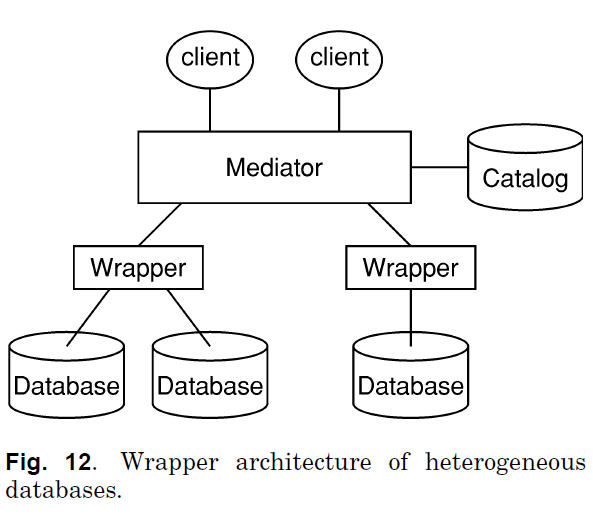
\includegraphics[width=\textwidth,height=0.5\textheight,keepaspectratio]{kossman-1.png} 
\footnote{\tiny{Изображение взято из \cite{Kossmann2000}}}
 \end{figure}    

\end{frame}

\begin{frame}
\frametitle{Описание возможностей участников}
\begin{itemize}
  \setlength\itemsep{1em}
  \item Описать возможности участников как views, хранить в каталоге. Гибок, но сложно реализовать;
  \item Capability records~--- КСГ-грамматика, описываем возможнсти \alert{запросов}. Используем их в генерации планов, нужны новые алгоритмы стоимостной и эвристической оптимизации;
\end{itemize}

\end{frame}

\begin{frame}
\frametitle{Оптимизация в гетерогенных РСУБД}

На примере правил обхода в системе Garlic (IBM)~\cite{Haas1997}.

\begin{itemize}
  \setlength\itemsep{1em}
  \item Идея: каждая обертка дает наружу набор правил (в виде функций) как с ней обращаться, что она умеет делать;
  \item Применяем стандартный алгоритм динамического программирования;
  \item Правила обхода (enumeration rules)~--- подаются в оптимизатор, получаем промежуточное представление, подаем его участникам, те транслируют в SQL и исполняют.
\end{itemize}

\end{frame}

\begin{frame}
\frametitle{Пример}

\begin{figure}[htb]
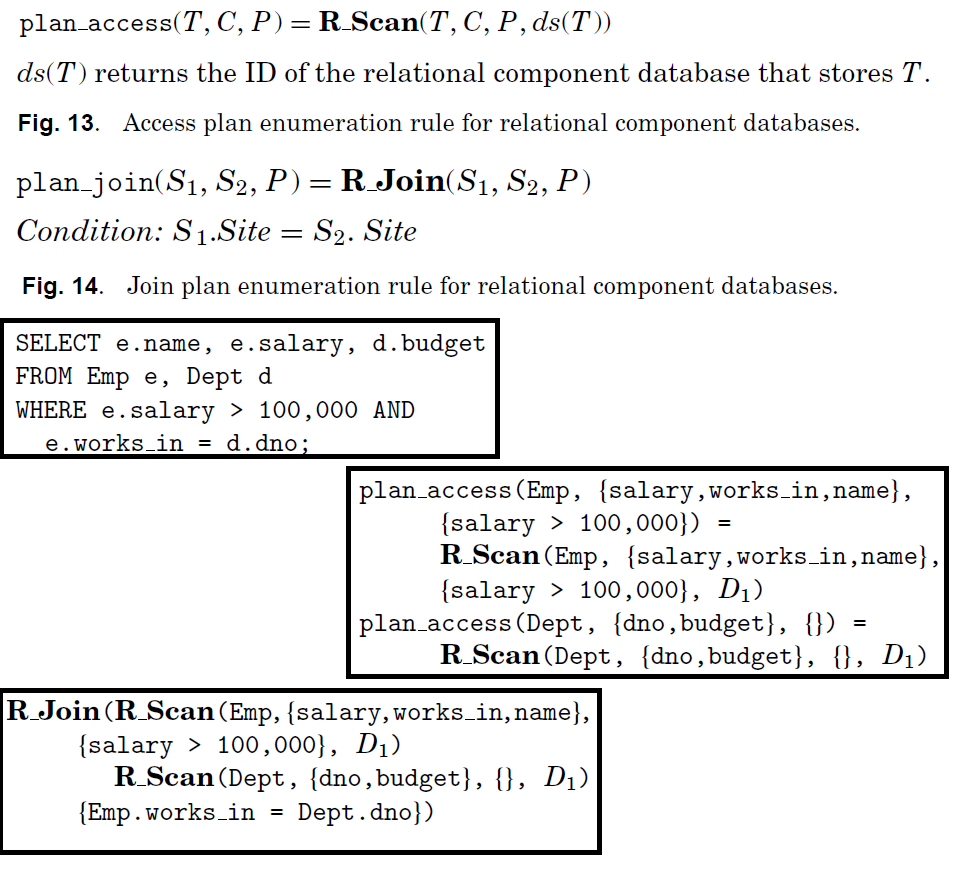
\includegraphics[width=\textwidth,height=0.80\textheight,keepaspectratio]{kossman-10.png} 
\footnote{\tiny{Изображение взято из \cite{Kossmann2000}}}
 \end{figure}    
\end{frame}

\begin{frame}
\frametitle{Плюсы подхода}

\begin{itemize}
  \setlength\itemsep{1em}
  \item Работает со стандартным стеком БД-технологий;
  \item Гибкость;
  \item Легко реализовывать;
  \item Итеративность разработки;
  \item Легкость добавления правил.
\end{itemize}
\end{frame}

\begin{frame}
\frametitle{Как получать статистику?}

\begin{itemize}
  \setlength\itemsep{1em}
  \item Калибровка: generic стоимостная модель
  $$n * c$$
  ищем $c$ с помощью тестовых запросов
  \begin{itemize}
    \item Модель~--- часть медиатора, писателям wrapper-ов не надо ее делать;
    \item Увы, не все компоненты можно описать такими моделями;
  \end{itemize}
  \item Правила + модель: точно, но трудно~--- каждому правилу сопоставляем формулу;
  \item Наблюдение + обучение: неточна, но можно делать адаптацию.
\end{itemize}

\end{frame}

\end{comment}

\begin{frame}[allowframebreaks]
\frametitle{Ссылки}
\footnotesize{
\begin{thebibliography}{99}


\bibitem[Elnikety, 2009] {Elnikety2009} Distributed DBMS. Sameh Elnikety. Encyclopedia of Database Systems. Ling Liu and M. Tamer {\"O}zsu (eds), p. 896--899. Springer US, 2009. \url{http://dx.doi.org/10.1007/978-0-387-39940-9\_654}

\bibitem[Kian-Lee Tan, 2009] {Kian-Lee2009} Distributed Database Systems. Kian-Lee Tan. Encyclopedia of Database Systems. Ling Liu and M. Tamer {\"O}zsu (eds), p. 894--896. Springer US, 2009. \url{http://dx.doi.org/10.1007/978-0-387-39940-9_701}

\bibitem[{\"O}zsu and Valduriez, 2009] {Ozsu2011} {\"O}zsu M.T. and Valduriez P. Principles of Distributed Database Systems, 3rd ed. Prentice-Hall, 2011.

\bibitem[Kossmann, 2000] {Kossmann2000} Donald Kossmann. 2000. The state of the art in distributed query processing. ACM Comput. Surv. 32, 4 (December 2000), 422--469. DOI=http://dx.doi.org/10.1145/371578.371598 

\bibitem[Haas et al., 1997] {Haas1997} Laura M. Haas, Donald Kossmann, Edward L. Wimmers, and Jun Yang. 1997. Optimizing Queries Across Diverse Data Sources. In Proceedings of the 23rd International Conference on Very Large Data Bases (VLDB '97). Morgan Kaufmann Publishers Inc., San Francisco, CA, USA, 276-285. 


%\bibitem[Ioannidis, 2003] {Ioannidis2003}  Yannis Ioannidis. 2003. The history of histograms (abridged). In Proceedings of the 29th international conference on Very large data bases - Volume 29 (VLDB '03), Johann Christoph Freytag, Peter C. Lockemann, Serge Abiteboul, Michael J. Carey, Patricia G. Selinger, and Andreas Heuer (Eds.), Vol. 29. VLDB Endowment 19--30. 

%\bibitem[Ioannidis and Poosala, 1995] {Ioannidis1995} Y. Ioannidis and V. Poosala. Histogram Based Solutions to Diverse Database Estimation Problems, IEEE Data Engineering, Vol. 18, No. 3, pp. 10--18, September 1995.

%\bibitem[Poosala et al., 1996] {Poosala1996} Viswanath Poosala, Peter J. Haas, Yannis E. Ioannidis, and Eugene J. Shekita. 1996. Improved histograms for selectivity estimation of range predicates. In Proceedings of the 1996 ACM SIGMOD international conference on Management of data (SIGMOD '96), Jennifer Widom (Ed.). ACM, New York, NY, USA, 294--305. DOI=http://dx.doi.org/10.1145/233269.233342 


%\bibitem[Kooi, 1980] {Kooi1980} Robert Philip Kooi. The Optimization of Queries in Relational Databases. PhD Thesis, Case Western Reserve University (1980).

%\bibitem[Piatetsky-Shapiro and Connel, 1984] {Piatetsky-Shapiro1984} Gregory Piatetsky-Shapiro and Charles Connell. 1984. Accurate estimation of the number of tuples satisfying a condition. In Proceedings of the 1984 ACM SIGMOD international conference on Management of data (SIGMOD '84). ACM, New York, NY, USA, 256--276. DOI=http://dx.doi.org/10.1145/602259.602294 


%\bibitem[Garcia-Molina et al., 2004] {Ulman2004} Гектор Гарсиа-Молина, Джеффри Д. Ульман, Дженнифер Уидом. Системы баз данных. Полный курс.  ISBN 5-8459-0384-Х; 2004 г. 

%\bibitem[Hellerstein et al., 2007] {Hellerstein2007} Joseph M. Hellerstein, Michael Stonebraker, and James Hamilton. Architecture of a Database System. Found. Trends databases 1, 2 (February 2007), 141--259. 

%\bibitem[Neumann, 2009] {Neumann2009} Thomas Neumann. Query Optimization (in Relational Databases). Encyclopedia of Database Systems. Springer US, 2009. 2273--2278.\url{http://dx.doi.org/10.1007/978-0-387-39940-9_293}

%\bibitem[Selinger et al., 1979] {Selinger1979} Selinger P.G., Astrahan M.M., Chamberlin D.D., Lorie R.A., and Price T.G. Access path selection in a relational database management System. In Proc. ACM SIGMOD Int. Conf. on Management of Data, 1979, pp. 23--34.

%\bibitem[Haas et al., 1989] {Haas1989} Haas L.M., Freytag J.C., Lohman G.M., and Pirahesh H. Extensible query processing in starburst. In Proc. ACM SIGMOD Int. Conf. on Management of Data, 1989, pp. 377--388.

%\bibitem[Graefe, 1995] {Graefe1995} Graefe G. The cascades framework for query optimization. Q. Bull. IEEE TC on Data Engineering, 18(3):19--29, 1995.

%\bibitem[Graefe and McKenna, 1993] {Graefe1993} Graefe G. and McKenna W.J. The volcano optimizer generator: Extensibility and efficient search. In Proc. 9th Int. Conf. on Data Engineering, 1993, pp. 209--218.

%\bibitem[Chaudhuri, 1998] {Chaudhuri1998} Chaudhuri S. An overview of query optimization in relational systems. In Proc. 17th ACM SIGACT-SIGMOD-SIGART Symp. Principles of Database Systems, 1998, pp. 34--43.

%\bibitem[Ioannidis, 1996] {Ioannidis1996} Ioannidis Y. Query optimization. In Handbook of Computer Science, A.B. Tucker (ed.). CRC Press, 1996.

%\bibitem[Jarke and Koch, 1984] {Chaudhuri1984} Jarke M. and Koch J. Query optimization in database systems. ACM Comput. Surv., 16(2):111–152, 1984.

%\bibitem[Ioannidis, 1996] {Ioannidis1996} Yannis E. Ioannidis. 1996. Query optimization. ACM Comput. Surv. 28, 1 (March 1996), 121--123. DOI=http://dx.doi.org/10.1145/234313.234367 

%\bibitem[Graefe, 1996] {Graefe1996} Goetz Graefe. 1996. Iterators, schedulers, and distributed-memory parallelism. Softw. Pract. Exper. 26, 4 (April 1996), 427--452. DOI=http://dx.doi.org/10.1002/(SICI)1097-024X(199604)26:4<427::AID-SPE20>3.3.CO;2-8 

\bibitem[Taniar et al., 2008] {Taniar2008} David Taniar, Clement H. C. Leung, Wenny Rahayu, and Sushant Goel. 2008. High Performance Parallel Database Processing and Grid Databases. Wiley Publishing. 

%\bibitem[Ramakrishnan and Gehrke, 2000] {Ramakrishnan2000}  Raghu Ramakrishnan and Johannes Gehrke. 2000. Database Management Systems (2nd ed.). Osborne/McGraw-Hill, Berkeley, CA, USA. 

\end{thebibliography}
}
\end{frame}


\end{document} 